\chapter{Хэрэгжүүлэлт}

Өмнөх бүлгүүдэд гаргасан ”UI”  болон ”UX" - ийн дизайниуд, системийн архитектур болон диаграммууд, шаардлагуудыг хэрэгжүүлж бүтээгдэхүүн болгон гаргасан үе шатуудын талаар энэхүү бүлэгтээ дурдана.
Хэрэгжүүлэлт хийх үе шатаа ерөнхийд нь задалвал:

\begin{itemize}
	\item Хөгжүүлэлтийн орчноо бэлдэх.
	\item Front-end хөгжүүлэлт.
	\item Back-end хөгжүүлэлт.
	\item Серверт байршуулах.
\end{itemize}

гэсэн алхмуудад хувааж гүйцэтгэсэн ба доор ажлуудаасаа гол гэсэн зүйлсээ нэгтгэн оруулав.

\section{Хөгжүүлэлтийн орчин}

Хэрэглэгч талд хэрэглэгдэх буюу ”Front-end” талын хэрэгжүүлэлтээ ”Next.js” технологи ашигласан ба харин ”Back-end” талын хөгжүүлэлтийг NodeJS, Socket.io ” технологи, өгөгдлөө ”Firebase” платформ дээр ”NoSQL” төрлөөр хадгалсан. Иймээс хөгжүүлэлтийн орчны хувьд ”Next.js” фрэймворкоо суулгаж, шаардлагатай тохиргоонуудыг хийж мөн адил NodeJS болон Socket.io”-ийг суулгаж, хэрэгтэй ашиглах сангуудаа татаж суулгаад, өгөгдлийн баазаа ”Firebase” дээр үүсгэж серверийг асаасан.

Хөгжүүлэлтийн явцын кодыг ”Github” болон ”Version Control” буюу ”Git” гэсэн технологиудыг сонгож хадгалсан ба хадгалах ”Repository” - ийг ”private” горимтой үүсгэсэн.

\clearpage
\begin{figure}[h]
	\centering
	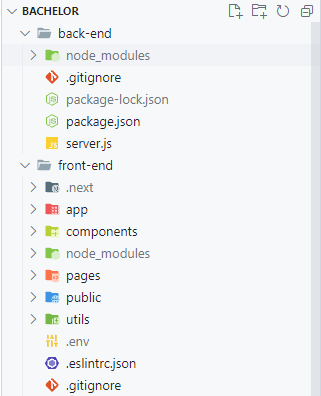
\includegraphics[width=10cm]{images/implement/file-structure.png}
	\caption{Төслийн файлын бүтэц}
	\label{fig:file-structure}
\end{figure}

Next.js дээр файлын бүтцээ Зураг 4.1 дээр харагдаж байгаачлан бүтэцлэж хөгжүүлэлтээ эхлэхэд бэлэн болголоо. Төслийн хувь "Back-end" талын хөгжүүлэлт "NodeJS" хэл дээр бичигдсэн учир төслийн хавтас маань хоёр салж "front-end", "back-end" гэж тусгаарлаж өгсөн. Файлын болон хавтсуудын бүтцийг тайлбарлавал

\begin{itemize}
	\item \textbf{backe-end/server.js} төслийн ”NodeJS” дээр бичигдсэн ”back-end” хэрэгжүүлэлтийн код байршина.
	\item \textbf{public} хавтаст ”front-end” төслийн хүрээнд ашиглах статик файлууд /зураг, icon/ байна.
	\item \textbf{component} хавтаст ”front-end” төслийн бүх компонент кодууд байршина.
	\item \textbf{app} хавтаст ”front-end” төслийн бүх хуудсууд, гол эх кодууд байршина.
	\item \textbf{pages/api/auth} Төсөлд хэрэглэгчийн хаяг, ”session”, ”authentication” зэргийг зохицуулах код байршина.
\end{itemize}

\section{Код хөгжүүлэлт}

Хөгжүүлэлтийн хувьд маш олон компонент, хуудсууд, тэдгээрийн код хийгдсэн тул хэрэглэгч шивэх үйл явцыг тайлбарлав.

\subsection{Гаргасан интерфэйс дээр тулгуурлаж гаргасан шивэх компонент хэсгийн хэрэгжүүлэлт}

Хамгийн эхлээд бэлдсэн хөгжүүлэлтийн орчин дээрээ хэрэглэгчийн шивэх үндсэн модал болон дотор нь ашиглаж буй компонентуудыг статик байдлаар өрөв.

\begin{lstlisting}[language=Javascript, caption=Хэрэглэгчийн мэдээллийг бодит хугацаанд харуулах компонент, frame=single]
  const PlayContent = (props: any) => {
    const { name, progress, wpm, completion, style } = props;
    return (
      <div className={`${style.playStatus} ${rubik.className}`}>
        <Typography
          variant="body1"
          fontSize={18}
          className={style.playStatusName}
        >
          {name}
        </Typography>
        <div className={style.progress_bar}>
          <div
            className={style.progress}
            style={{ width: `${progress}%` }}
          ></div>
        </div>
        <div className={style.playContentEnd}>
          <Typography
            variant="body1"
            fontSize={18}
            className={style.playContentBodyText}
          >
            {wpm}WPM
          </Typography>
          <Typography
            variant="body1"
            fontSize={18}
            className={style.playContentBodyText}
          >
            {completion}%
          </Typography>
        </div>
      </div>
    );
  };
			
\end{lstlisting}

Мэдээлэлд тоглогчийн нэр (name), хувь (progress), минут тутамд үг (wpm), гүйцэтгэлийн хувь (accuracy) зэрэг орно.

\subsection{Client хэсгийн Socket.io өрөө үүсгэх, орж буй хэрэгжүүлэлт}

Уралдааны хуудас рэндэр хийгдэх үед Socket ашиглан unique өрөөг үүсэх. Хэрвээ үүссэн өрөөнд орох бол URL аас param ийг шалган өрөөнд нэвтрүүлнэ.

\begin{lstlisting}[language=Javascript, caption=Хэрэглэгч өрөөнд нэвтрэх client талын код, frame=single]
	useEffect(() => {
    const socket = io("https://typeracer-ytd7.onrender.com");
    setSocket(socket);
    const setupSocket = () => {
      if (searchParams!.get("roomId")) {
        const roomId = searchParams!.get("roomId");
        socket!.emit("join-room", roomId);

        socket.on("room-joined", (userCount, roomTextId) => {
          // setTextId(roomTextId);
        });
      } else {
        socket!.emit("create-room", textId);
      }

      return () => {
        socket!.disconnect();
      };
    };

    setupSocket();
  }, [textId]);
			
\end{lstlisting}


\subsection{Өгөгдлийн сангаас текст харуулах функц}

Өрөөнд амжилттай орсон үед баазаас race\_text гэх json оос санамсаргүй байдлаар сонгон авч useEffect ашиглан текстийн талбарт оноож өгнө.
useEffect нь empty massive хамаарлын ([]) заасны дагуу бүрэлдэхүүнийг холбох үед нэг удаа ажиллаж өгөгдлийг дуудаж, боловсруулдаг.

\begin{lstlisting}[language=Javascript, caption=Текст fetch хийж буй async функц, frame=single]
	useEffect(() => {
    const fetchData = async () => {
      try {
        const race_text = await fetch(
          "https://typeracer-1be53-default-rtdb.asia-southeast1.firebasedatabase.app/race_text.json"
        );

        const race = await fetch(
          "https://typeracer-1be53-default-rtdb.asia-southeast1.firebasedatabase.app/race.json"
        );

        const user_statistics = await fetch(
          "https://typeracer-1be53-default-rtdb.asia-southeast1.firebasedatabase.app/user_statistics.json"
        );

        if (race_text.ok) {
          const data = await race_text.json();
          const id = Math.floor(Math.random() * data.length);
          const quote = data[id];

          setTextId(id);
          setWords(quote.content);
        } else {
          console.error(
            `Error: Unable to fetch data. Status Code: ${race_text.status}`
          );
        }
        if (race.ok) {
          const race_data = await race.json();
          const raceId = race_data.length;
          setRaceId(raceId);
        }
        if (user_statistics.ok) {
          const user_data = await user_statistics.json();
          const userId = user_data.length;
          setUserId(userId);
        }
      } catch (error) {
        console.error("Error fetching data:", error);
      }
    };
    fetchData();
  }, []);
			
\end{lstlisting}

\subsection{Firebase тохиргоо}

Firebase Config нь хэрэглэгчээс програмын шинэчлэлтийг татаж авах шаардлагагүйгээр өөрийн апп-ын төлөв байдал, харагдах байдлыг өөрчлөх боломжийг олгодог.
Энэхүү код нь Firebase програм, бодит цагийн өгөгдлийн санг (db) болон баталгаажуулалтын жишээг (auth) програмын бусад хэсэгт ашиглахаар экспортолно.

\begin{lstlisting}[language=Javascript, caption=Firebase config, frame=single]
	import { getApp, getApps, initializeApp } from "firebase/app";
	import { getDatabase } from "firebase/database";
	import { getAuth } from "firebase/auth";

	const firebaseConfig = {
		apiKey: process.env.NEXT_PUBLIC_FIREBASE_API_KEY,
		authDomain: process.env.NEXT_PUBLIC_FIREBASE_AUTH_DOMAIN,
		databaseURL: process.env.NEXT_PUBLIC_FIREBASE_DATABASE_URL,
		projectId: process.env.NEXT_PUBLIC_FIREBASE_PROJECT_ID,
		storageBucket: process.env.NEXT_PUBLIC_FIREBASE_STORAGE_BUCKET,
		messagingSenderId: process.env.NEXT_PUBLIC_FIREBASE_MESSAGING_SENDER_ID,
		appId: process.env.NEXT_PUBLIC_FIREBASE_APP_ID,
	};

	const firebaseApp = getApps().length ? getApp() : initializeApp(firebaseConfig);
	const db = getDatabase(firebaseApp);
	const auth = getAuth();

export { firebaseApp, db, auth };

\end{lstlisting}

\subsection{Тоглоомын удирдах hook}

Энэхүү useEffect hook нь статус дээр тулгуурлан янз бүрийн зан үйлийг удирддаг. Статус "playing" үед setInterval-ийг ашиглан цагийн хязгаарыг тохируулж, TIME\_LIMIT хүрэх хүртэл цагийн төлөвийг секунд тутамд нэмэгдүүлнэ. Хэрэв статус "completed" эсвэл "finished" бол энэ нь интервалыг арилгаж, төлөвийг шинэчилж, горимыг харуулж, тохируулсан функцийг ашиглан Firebase бодит цагийн мэдээллийн сан дахь өгөгдлийг шинэчилдэг.

\begin{lstlisting}[language=Javascript, caption=Тоглоомын цагийг удирдах Firebase өгөгдлийг шинэчлэхэд зориулсан useEffect hook, frame=single]
  useEffect(() => {
    let timeLimit: any;
    if (status === "playing") {
      if (inputRef.current) {
        inputRef.current.focus();
      }
      timeLimit = setInterval(() => {
        setTime((prev) => {
          if (prev >= TIME_LIMIT) {
            clearInterval(timeLimit);
            setStatus("finished");
            return TIME_LIMIT;
          } else {
            return prev + 1;
          }
        });
      }, 1000);
    } else if (status === "completed") {
      clearInterval(timeLimit);
      setFailed(false);
      setShowModal(true);

      set(ref(db, "race/" + raceId), {
        creator_id: session?.data?.user?.email,
        race_type_id: 1,
        text_id: textId,
        created_at: Date.now(),
        updated_at: Date.now(),
      });

      set(ref(db, "user_statistics/" + userId), {
        user_id: session?.data?.user?.email,
        avg_wfm: calculateWPM(time, wordIndex).currentWPM,
        avg_accuracy: calculateAccuracy(correct, wrong),
        highest_wpm: calculateWPM(time, wordIndex).highestWPM,
        lowest_wpm: calculateWPM(time, wordIndex).lowestWPM,
        created_at: Date.now(),
        updated_at: Date.now(),
      });
    } else if (status === "finished") {
      clearInterval(timeLimit);
      setFailed(true);
      setShowModal(true);

      set(ref(db, "race/" + raceId), {
        creator_id: session?.data?.user?.email,
        race_type_id: 1,
        text_id: textId,
        created_at: Date.now(),
        updated_at: Date.now(),
      });

      set(ref(db, "user_statistics/" + userId), {
        user_id: session?.data?.user?.email,
        avg_wfm: calculateWPM(time, wordIndex).currentWPM,
        avg_accuracy: calculateAccuracy(correct, wrong),
        highest_wpm: calculateWPM(time, wordIndex).highestWPM,
        lowest_wpm: calculateWPM(time, wordIndex).lowestWPM,
        created_at: Date.now(),
        updated_at: Date.now(),
      });
    }

    return () => clearInterval(timeLimit);
  }, [status]);
			
\end{lstlisting}


\subsection{Next-Auth ашиглаж хэрэглэгчийн Authentication, Session зохицуулах}

Цахим шуудан болон нууц үг ашиглан баталгаажуулалтын процессыг хариуцдаг "Credentials" нэртэй тусгай баталгаажуулалтын үйлчилгээг зааж өгч, NextAuth болон Firebase ашиглаж хэрэглэгчийн Authenticationийг зохицуулсан.

\begin{lstlisting}[language=Javascript, caption= Хэрэглэгчийн Authentication болон Session-г зохицуулах, frame=single]
	export const authOptions = {
		pages: {
			signIn: "/login",
		},
	
		providers: [
			CredentialsProvider({
				name: "Credentials",
				credentials: {},
				async authorize(credentials): Promise<any> {
					return await signInWithEmailAndPassword(
						auth,
						(credentials as any).email || "",
						(credentials as any).password || ""
					)
						.then((userCredential) => {
							if (userCredential.user) {
								return userCredential.user;
							}
							return null;
						})
						.catch((error) => console.log(error))
						.catch((error) => {
							const errorCode = error.code;
							const errorMessage = error.message;
							console.log(error);
						});
				},
			}),
		],
	};
	
	export default NextAuth(authOptions);
	
\end{lstlisting}


\subsection{Socket.io болон ExpressJS ашигласан back-end талын хөгжүүлэлт}

Энэхүү Node.js серверийн код нь хэрэглэгч хоорондох бодит цагийн харилцааг удирдахын тулд Socket.IO санг ашигласан. Энэ нь хэрэглэгчдэд өрөө бүрийг санамсаргүй ID-аар тодорхойлсон өрөө үүсгэх, нэгдэх боломжийг олгоно. Сервер нь өрөө тус бүрд холбогдсон хэрэглэгчдийг хянаж, өрөө үүсгэх, нэгдэх үйл явдлуудыг зохицуулж, хэрэглэгчид гарах үед өрөөг устгадаг.

\begin{lstlisting}[language=Javascript, caption=Socket ашиглан хэрэглэгчдийг зохицуулах, frame=single]
	
io.on("connection", (socket) => {
  console.log("A user connected: " + socket.id);

  socket.on("create-room", (textId) => {
    const roomId = Math.random().toString(36).substring(2, 7);

    socket.join(roomId);

    roomUsers[roomId] = {
      textId: textId,
      users: [],
    };
    roomUsers[roomId].users.push(socket.id);
    console.log(`User created and joined room ${roomId}`);

    io.to(roomId).emit("room-created", roomId);
    console.log(roomUsers);
  });

  socket.on("join-room", (roomId) => {
    socket.join(roomId);
    console.log(roomUsers);

    if (!roomUsers[roomId]) {
      roomUsers[roomId] = { textId: 0, users: [] };
    }

    roomUsers[roomId].users.push(socket.id);

    io.to(roomId).emit(
      "room-joined",
      roomUsers[roomId].users.length,
      roomUsers[roomId].textId
    );

    console.log(`${roomId} өрөөнийхөн ${roomUsers[roomId].users}`);
  });

  socket.on("disconnect", () => {
    console.log("User disconnected");
    Object.keys(roomUsers).forEach((room) => {
      roomUsers[room].users = roomUsers[room].users.filter(
        (user) => user !== socket.id
      );
      console.log(
        `Users in room ${room} after disconnect:`,
        roomUsers[room].users
      );

      if (roomUsers[room].users.length === 0) {
        delete roomUsers[room];
      }
    });
  });
});

\end{lstlisting}


\subsection{Серверт байршуулах}

Хийсэн төслийнхөө эцсийн хувилбарыг онлайн хэлбэрээр серверт байршуулж хэрэглэгчид шууд ашиглах боломжтой байдаар cерверт байршуулсан ба төслийнхөө ”Front-end” хэсгийг ”Vercel.com” дээр байршуулсан бөгөөд хэрэглэгч хүсэлт илгээхэд ”Back-end” серверээс зохицуулалт хийж хүсэлтэд хариулт илгээж байх ёстой учир тусдаа сервер дээр ”Backend” хэсгийн кодоо render.com дээр асаав.


\begin{itemize}
	\item \textbf{Website link:} \url{https://duckrace.vercel.app/}
\end{itemize}